\chapter{Постановка задачи}
\label{sec:problem_formulation}

Предположим, что трещина гидроразрыва пласта (ГРП) развивается в слоистом пласте под действием давления закачиваемой через скважину жидкости. Будем считать, что пласт является слоистым в вертикальном направлении, но каждый слой представляет собой однородную изотропную линейно упругую среду, обладающую своими модулями упругости. В силу того, что горная порода находится под давлением вышележащих масс, в каждом слое имеются свои сжимающие напряжения. Как правило, тензор напряжений устроен таким образом, что максимальным является вертикальное напряжение, а два других главных напряжения сонаправлены во всех слоях, но имеют различные по модулю величины. Трещина раскрывается в вертикальной плоскости вдоль вектора максимального горизонтального главного напряжения, преодолевая минимальные горизонтальные напряжения.

\section{Математическая формулировка}

Введем систему координат расположив ее начало в центре закачки жидкости (скважина), ось $Oy$ --- вдоль вертикального направления, ось $Ox$ вдоль плоскости трещины в горизонтальном направлении и ось $Oz$ --- поперек трещины (рисунок~\ref{fig:planar_fracture}). Сжимающие напряжения, действующие поперек плоскости трещины в $i$-м слое обозначим через $\sigma_h^i$.

\begin{figure}[htbp]
    \centering
    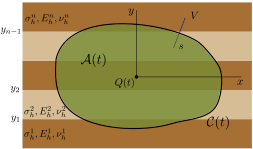
\includegraphics[width=0.7\textwidth]{fracture_scheme.pdf}
    \caption{Модель плоской трещины.}
    \label{fig:planar_fracture}
\end{figure}

Уравнение неразрывности в приближении тонкого слоя для движения жидкости внутри плоской трещины  имеет вид
\begin{equation}
    \label{eq:conservation_law}
    \pd{w}{t} + \bigtriangledown \cdot \mathbf{q} + \frac{2C_L}{\sqrt{t-t_0(x,\, y)}}  = Q(t) \delta(x,\,y),
\end{equation}
где $w(x,y,t)$ --- раскрытие трещины, $\mathbf{q}(x,y,t)$ --- поток жидкости внутри трещины, $Q(t)$ --- расход закаченной в трещину жидкости. Фильтрационные утечки жидкости из трещины в пласт вычисляются согласно модели Картера~\cite{Cart1957}, $t_0(x,\, y)$ --- момент времени, в который фронт трещины достиг точки $(x, y)$.

Используя закон Пуазейля $\mathbf{q}  = -\frac{w^3}{12\mu} \bigtriangledown\! p$ получим уравнение Рейнольдса \cite{DONTSOV201753}
\begin{equation}
    \label{eq:reynolds_equation}
    \pd{w}{t} - \text{div} \left(\frac{w^3}{12\mu} \bigtriangledown \!p \right) + \frac{2C_L}{\sqrt{t-t_0(x,\, y)}}  = Q(t) \delta(x,\,y),
\end{equation}
где $\mu$ --- вязкость жидкости, $p(x,y,t)$ --- давление жидкости, действующее на поверхности трещины.

Связь раскрытия трещины $w$ с давлением жидкости $p$ задается уравнением упругости
\begin{equation}
    \label{eq:elasticity_equation}
    p(x,y,t) = \sigma_h(y) + \int\limits_{\mathcal{A}(t)} G(x,y;x',y')w(x',y',t) \dif x' \dif y',
\end{equation} 
где $\mathcal{A}(t)$ --- площадь плоской трещины, $\sigma_h$ --- сжимающие напряжение. В случае изотропной среды
\begin{equation}
    \label{eq:elasticity_kernel}
    G(x,y;x',y') = - \frac{E'}{8\pi [(x\!-\!x')^2+(y\!-\!y')^2]^{3/2}}.
\end{equation}
$E' = E / (1-\nu^2)$, где $E$ --- модуль Юнга, $\nu$ --- коэффициент Пуассона.

В случае неоднородности модулей упругости по слоям ядро $G(x,y;x',y')$ не имеет аналитического вида, и для его нахождения требуется численное построение.

Задача моделирования раскрытия трещины ГРП состоит в решении интегро-дифференциального уравнения, получаемого подстановкой выражения для давления из уравнения~\eqref{eq:elasticity_equation} в уравнение Рейнольдса~\eqref{eq:reynolds_equation} при заданном расходе жидкости $Q(t)$. Сложность решения состоит в вырожденности получаемого уравнения на фронте трещины (при $w=0$) и необходимости определять динамику фронта трещины (задача со свободной границей).

\section{Численная постановка}

Дискретизация уравнений \eqref{eq:reynolds_equation} и \eqref{eq:elasticity_equation} осуществляется с помощью метода разрывных смещений (МРС) \cite{dispalecement_discontinuty_Crouch1983}. Для этого часть плоскости, внутри которой мы предполагаем раскрытие трещины, разбивается на элементы $\mathcal{A}_{i,j}$ с помощью прямоугольной сетки. Центр ячейки $\mathcal{A}_{i,j}$ расположен в $(x_i,y_j)$ и имеет размеры $\Delta x$, $\Delta y$. Для раскрытия трещины $w$ и давления $p$ используется кусочно-постоянная аппроксимация
\begin{equation}
    \label{eq:piecewiece_approximation}
    \begin{split}
        w(x,y,t) &= \sum\limits_{i,j} w_{i,j}(t) H_{i,j}(x,y), \\
        p(x,y,t) &= \sum\limits_{i,j} p_{i,j}(t) H_{i,j}(x,y), \\
    \end{split}
\end{equation}
где 
\begin{equation}
    \label{eq:heaviside_function}
    H_{i,j}(x,y) = \left\{
        \begin{array}{ll}
            1, & (x,y) \in \mathcal{A}_{i,j}, \\
            0, & (x,y) \notin \mathcal{A}_{i,j}.
        \end{array}\right.
\end{equation}

Тогда уравнение упругости \eqref{eq:elasticity_equation} путём явного интегрирования по элементу $\mathcal{A}_{i,j}$ сводится к
\begin{equation}
    \label{eq:discrete_elasticity}
    p_{i,j}(t) = {\sigma_h}_{i,j} + \sum\limits_{k,l} C_{i,j;k,l} w_{k,l}(t),
\end{equation}
где $C_{i,j;k,l}$ -- матрица упругости. Дискретизация уравнения Рейнольдса \eqref{eq:reynolds_equation} осуществляется путем интегрирования по времени и элементу. В целом, алгоритм решения задачи \cite{DONTSOV201753} является достаточно сложным и приведен в Приложении~\ref{app:discrete-reynolds}.